\chapter{Систем хөгжүүлэх онол, арга зүйн судалгаа}

\section{Системийн тухай танилцуулга}

Сүүлийн жилүүдэд ахлах сургуулийн сурагчид гадаадын их, дээд сургуульд элсэх
сонирхол нэмэгдэхийн зэрэгцээ элсэлтийн материал бүрдүүлэлт, хугацааны удирдлага,
даалгаврын хяналт болон зөвлөх багштай харилцах үйл ажиллагааг илүү зохион
байгуулалттайгаар удирдах хэрэгцээ нэмэгдэж байна. Гэвч одоогийн байдлаар ихэнх
сургууль болон зөвлөх байгууллага элсэлтийн процессыг и-мэйл, excel файл,
цаасан материал болон олон төрлийн салангид платформ ашиглан удирддаг нь
мэдээлэл алдагдах, хугацаа хоцрох, даалгаврын явцыг хянахад хүндрэл үүсгэх
асуудлуудыг бий болгож байна.

Иймээс энэхүү төслийн хүрээнд ахлах сургуулийн сурагчдын гадаадын их
сургуульд элсэх бэлтгэл үйл явцыг нэгдсэн платформоор удирдах веб системийг
хөгжүүлэхээр зорьсон. Уг систем нь сурагч, зөвлөх багш, багш, сургуулийн админ
болон super admin зэрэг олон төрлийн хэрэглэгчийн эрхтэйгээр ажиллах бөгөөд
даалгавар удирдах, материал солилцох, бодит цагийн чат ашиглах, элсэлтийн
үр дүн хянах, хиймэл оюунд суурилсан сургуулийн зөвлөмж өгөх зэрэг боломжуудыг агуулна.

Системийн үндсэн зорилго нь сурагч болон зөвлөх багшийн хоорондын
харилцааг илүү үр ашигтай болгох, элсэлтийн материал бүрдүүлэх явцыг хянах, мэдээллийг төвлөрсөн байдлаар хадгалах, мөн сурагчдын гүйцэтгэлийг
сайжруулахад оршино.

Систем нь Next.js framework, MongoDB өгөгдлийн сан, JWT authentication,
Vercel cloud infrastructure зэрэг орчин үеийн веб технологиуд дээр суурилан
хөгжүүлэгдсэн.

\section{Хэрэглэгчийн судалгаа}

Системийн шаардлагыг тодорхойлох зорилгоор гадаадын их, дээд сургуульд
элсэх бэлтгэл хийж буй сурагчид болон зөвлөх багш нартай ярилцлага
хэлбэрийн судалгаа хийсэн. Судалгааны хүрээнд зөвлөх багш нарын өдөр
тутмын үйл ажиллагаа, сурагчдын материал бүрдүүлэлт, даалгаврын хяналт
болон харилцааны үеийн хүндрэлүүдийг тодорхойлохыг зорьсон.

Ярилцлагын үр дүнд дараах нийтлэг асуудлууд илэрсэн. Үүнд:

\begin{itemize}
\item Сурагчдын даалгавар болон материал бүрдүүлэлтийн явцыг нэгдсэн
байдлаар хянах боломж хязгаарлагдмал байдаг;

\item Даалгаврын хугацаа болон шаардлагатай материалуудыг и-мэйл,
чат болон excel файл ашиглан удирддаг тул мэдээлэл алдагдах,
мартагдах асуудал үүсдэг;

\item Зөвлөх багш нэгэн зэрэг олон сурагчтай ажиллах үед сурагч бүрийн
гүйцэтгэлийн явцыг хянахад хүндрэлтэй байдаг;

\item Тодорхойлох захидал бичих хүсэлт болон материал солилцоо
эмх цэгцгүй явагддаг;

\item Сурагч болон зөвлөх багшийн хоорондын харилцаа олон төрлийн
платформ дээр явагддаг тул мэдээллийн нэгдмэл байдал алдагддаг;

\item Элсэлтийн материалуудын сүүлийн хувилбарууд холилдох,
алдаатай файл илгээх асуудал түгээмэл тохиолддог;

\item Сурагчдад тохирох сургуулийг сонгох үйл явц нь ихэвчлэн гар
аргаар явагддаг тул цаг хугацаа их шаарддаг.
\end{itemize}

\begin{figure}[H]
\centering
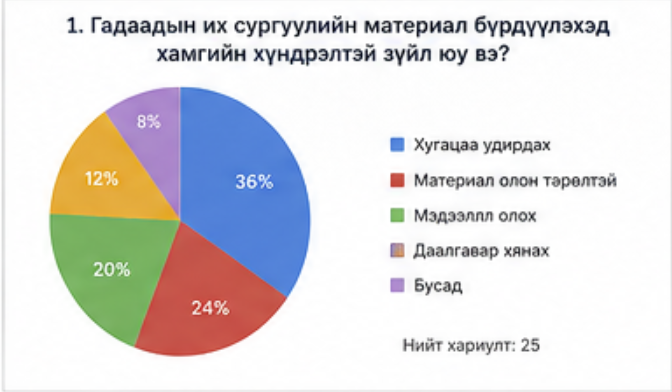
\includegraphics[width=0.5\textwidth]{Figures/chapter1/sudalgaa1.png}
\caption{Хэрэглэгчийн судалгааны үр дүн}
\end{figure}

Зураг 1.1-ээс харахад гадаадын их сургуулийн материал бүрдүүлэх явцад
оролцогчдын хувьд хугацаа удирдах асуудал хамгийн их хүндрэл үүсгэж байна.
Мөн материал олон төрөлтэй байх, шаардлагатай мэдээллийг цаг тухайд нь
олж авах, даалгаврын явцыг хянах зэрэг асуудлууд давхар илэрсэн. Иймээс
системийн шаардлагад зөвхөн баримт бичиг хадгалах боломж бус, харин хугацаа,
даалгавар, материалын төлөвийг нэг дороос хянах зохион байгуулалт зайлшгүй
шаардлагатай гэж үзэв.

\begin{figure}[H]
\centering
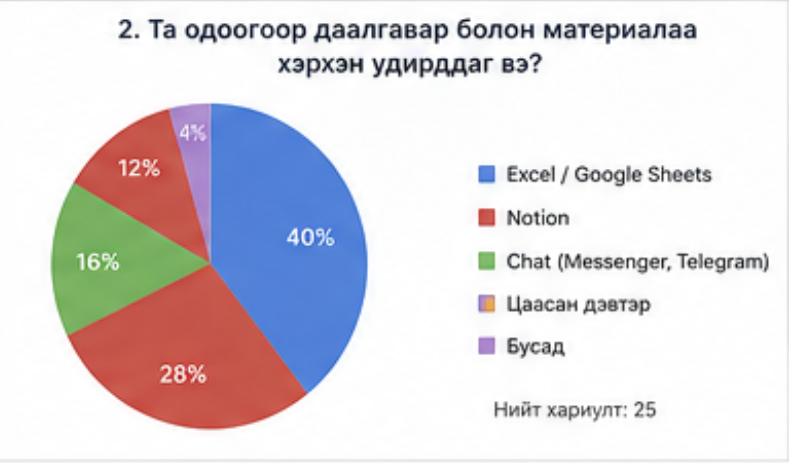
\includegraphics[width=0.5\textwidth]{Figures/chapter1/sudalgaa2.png}
\caption{Хэрэглэгчийн судалгааны үр дүн}
\end{figure}

Зураг 1.2-т оролцогчид даалгавар болон материалаа одоогоор ихэвчлэн
Excel, Google Sheets, Notion, чат болон бусад салангид хэрэгслээр удирдаж
байгааг харуулж байна. Эдгээр хэрэгслүүд нь тодорхой хэмжээнд ашиглахад
хялбар боловч элсэлтийн материалын хувилбар, даалгаврын төлөв, сануулга,
харилцааны түүхийг нэг бүтцэд нэгтгэхэд хангалтгүй. Ийм нөхцөл нь мэдээлэл
давхцах, сүүлийн хувилбар тодорхойгүй болох, зөвлөх багш олон сурагчийн
явцыг зэрэг хянахад хүндрэл үүсгэх үндсэн шалтгаан болж байна.

\begin{figure}[H]
\centering
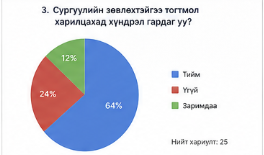
\includegraphics[width=0.5\textwidth]{Figures/chapter1/sudalgaa3.png}
\caption{Хэрэглэгчийн судалгааны үр дүн}
\end{figure}

Зураг 1.3-т сургуулийн зөвлөхтэй тогтмол харилцах хэрэгцээ өндөр байгааг
харуулсан бөгөөд оролцогчдын дийлэнх нь ийм төрлийн харилцаа шаардлагатай
гэж үзсэн байна. Энэ үр дүн нь системд зөвлөх багш, сурагчийн хоорондын
шуурхай мэдээлэл солилцоо, мэдэгдэл, хүсэлт илгээх болон даалгаврын явцын
эргэх холбоог дэмжих функцүүдийг тусгах үндэслэл болж байна.

Дээрх ярилцлага болон судалгааны үр дүнг нэгтгэн үзэхэд хэрэглэгчдийн
гол хүндрэл нь даалгаврын явц хянах, элсэлтийн баримт бичиг солилцох,
зөвлөх багш болон сурагчийн харилцааг нэг сувгаар зохион байгуулах,
мөн хугацааны сануулгыг тогтмол авах хэрэгцээнд төвлөрч байна. Иймээс
системийн шаардлагад task tracking, document exchange, counselor-student
communication болон deadline reminder функцүүдийг үндсэн бүрэлдэхүүн
хэсэг болгон тусгах нь зүйтэй гэж үзэв.

Судалгааны үр дүнгээс харахад сурагч болон зөвлөх багшийн хоорондын
харилцаа, даалгаврын удирдлага, материал бүрдүүлэлт болон элсэлтийн
явцыг нэгдсэн байдлаар удирдах веб систем шаардлагатай байгаа нь
харагдсан.

\subsection{SMART зарчим}

Системийн шаардлагыг тодорхойлохдоо SMART зарчмыг баримталсан.

\begin{itemize}
\item Specific – Сурагч болон зөвлөх багшийн даалгавар, материал болон харилцааг нэг системд төвлөрүүлэх
\item Measurable – Даалгаврын гүйцэтгэл болон материал бүрдүүлэлтийн явцыг хувиар хэмжих
\item Achievable – Next.js болон MongoDB технологи ашиглан хэрэгжүүлэх боломжтой
\item Relevant – Гадаадын их сургуулийн элсэлтийн процессыг илүү үр ашигтай удирдах шаардлагад нийцсэн
\item Time-bound – Системийн үндсэн хөгжүүлэлтийг 2026 оны 5-р сар хүртэл гүйцэтгэх
\end{itemize}



\section{Ижил төстэй системийн судалгаа}

Энэхүү системтэй төстэй олон улсын болон дотоодын системүүдийг судалж, тэдгээрийн онцлог, давуу болон сул талуудыг харьцуулсан.

\subsection{Scoir систем}

Scoir нь АНУ-д өргөн ашиглагддаг коллежийн зөвлөгөөний платформ бөгөөд ахлах сургуулийн сурагчдад их сургуулийн сонголт хийх,
материал бүрдүүлэх болон элсэлтийн процессыг удирдах боломжийг олгодог
веб систем юм. Тус систем нь сурагч, зөвлөх багш болон эцэг эхийн хамтын
оролцоонд тулгуурласан бүтэцтэйгээр хөгжүүлэгдсэн байдаг.

Scoir системийн гол онцлог нь сурагчийн академик үзүүлэлт, сонирхол,
гадуурх үйл ажиллагаа болон карьерын чиглэлийг харгалзан тохирох их
сургуулиудыг санал болгодог university matching механизм юм. Мөн
сурагч бүрийн application progress, материал бүрдүүлэлт болон deadline-ийг
нэгдсэн dashboard орчноос хянах боломжтой.

Түүнчлэн зөвлөх багш нь сурагч бүрийн элсэлтийн явцыг хянах, зөвлөгөө өгөх,
материал шалгах болон communication хийх боломжтой байдаг. Scoir систем нь
document management, messaging, application tracking болон recommendation
зэрэг боломжуудыг нэг платформд нэгтгэсэнээрээ онцлогтой.

Гэвч Scoir систем нь Монголын сургуулийн орчинд шууд ашиглахад зарим
хязгаарлалттай байдаг. Үүнд:
\begin{itemize}
\item Монгол хэлний дэмжлэггүй;
\item Монгол сургуулийн workflow болон зөвлөх үйлчилгээний бүтэцтэй бүрэн таардаггүй;
\item Subscription болон ашиглалтын зардал өндөр;
\item Системийн зарим боломжууд зөвхөн АНУ-ын их сургуулийн admission системд төвлөрсөн;
\item Өөрөө удирдах боломж хязгаарлагдмал.
\end{itemize}

Эдгээрээс харахад Scoir нь их сургуулийн элсэлтийн зөвлөгөө талдаа илүү хөгжсөн
систем боловч Монголын ахлах сургуулийн орчинд тохируулан ашиглах боломжгүй байсан.

\begin{figure}[H]
\centering
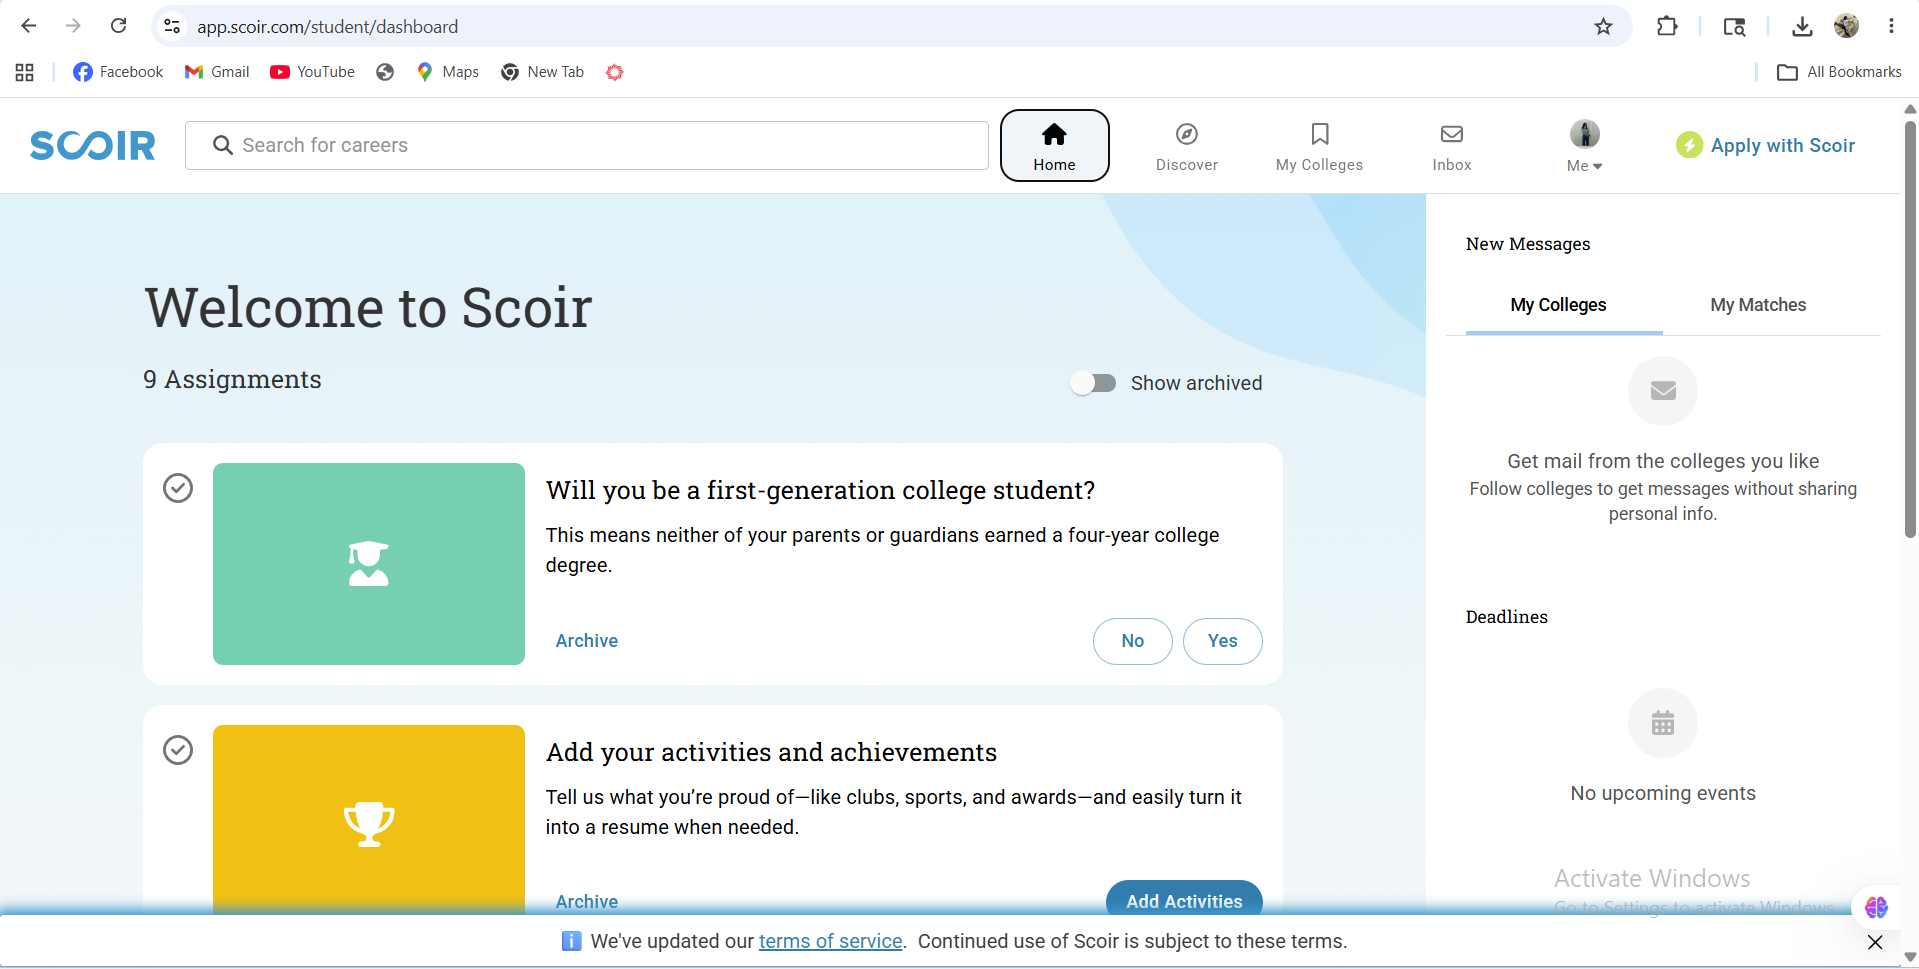
\includegraphics[width=0.9\textwidth]{Figures/chapter1/scoir.png}
\caption{Scoir системийн dashboard интерфейс}
\end{figure}

\subsection{BridgeU систем}

BridgeU нь Их Британид хөгжүүлэгдсэн university guidance болон career
planning платформ бөгөөд сурагчдад өөрийн сонирхол, ур чадвар болон
академик үзүүлэлтэд тохирсон их сургуулийг сонгоход туслах зориулалттай
систем юм.

Тус систем нь AI recommendation болон university matching механизм
ашиглан сурагчийн профайлд үндэслэн тохирох сургуулиудыг санал болгодог.
Мөн application tracking, карьерын тест, deadline management болон
counselor communication зэрэг боломжуудыг агуулдаг.

BridgeU системийн нэг давуу тал нь сурагчийн career pathway болон
сонирхлын мэдээллийг ашиглан урт хугацааны төлөвлөлт хийх боломжийг
олгодог явдал юм. Зөвлөх багш нь сурагч бүрийн application progress,
career interest болон материал бүрдүүлэлтийн явцыг хянах боломжтой байдаг.

Мөн систем нь их сургуулийн мэдээллийн сан, scholarship information болон
admission requirement мэдээллийг төвлөрсөн байдлаар харуулах боломжтой.

Гэвч судалгааны үр дүнд дараах сул талууд ажиглагдсан. Үүнд:

\begin{itemize}
\item Real-time chat болон шууд харилцааны боломж хязгаарлагдмал;
\item Даалгаврын удирдлагын модуль харьцангуй энгийн;
\item Монгол хэл болон Монгол сургуулийн орчинд тохирсон localization байхгүй;
\item Системийн зарим premium боломжууд өндөр төлбөртэй;
\item Custom workflow боловсруулах боломж хязгаарлагдмал.
\end{itemize}

Иймээс BridgeU систем нь university recommendation болон career planning
чиглэлд хүчтэй боловч Монголын сургуулийн admission workflow болон
зөвлөх үйлчилгээний онцлогт бүрэн нийцэхгүй байгаа нь ажиглагдсан.

\begin{figure}[H]
\centering
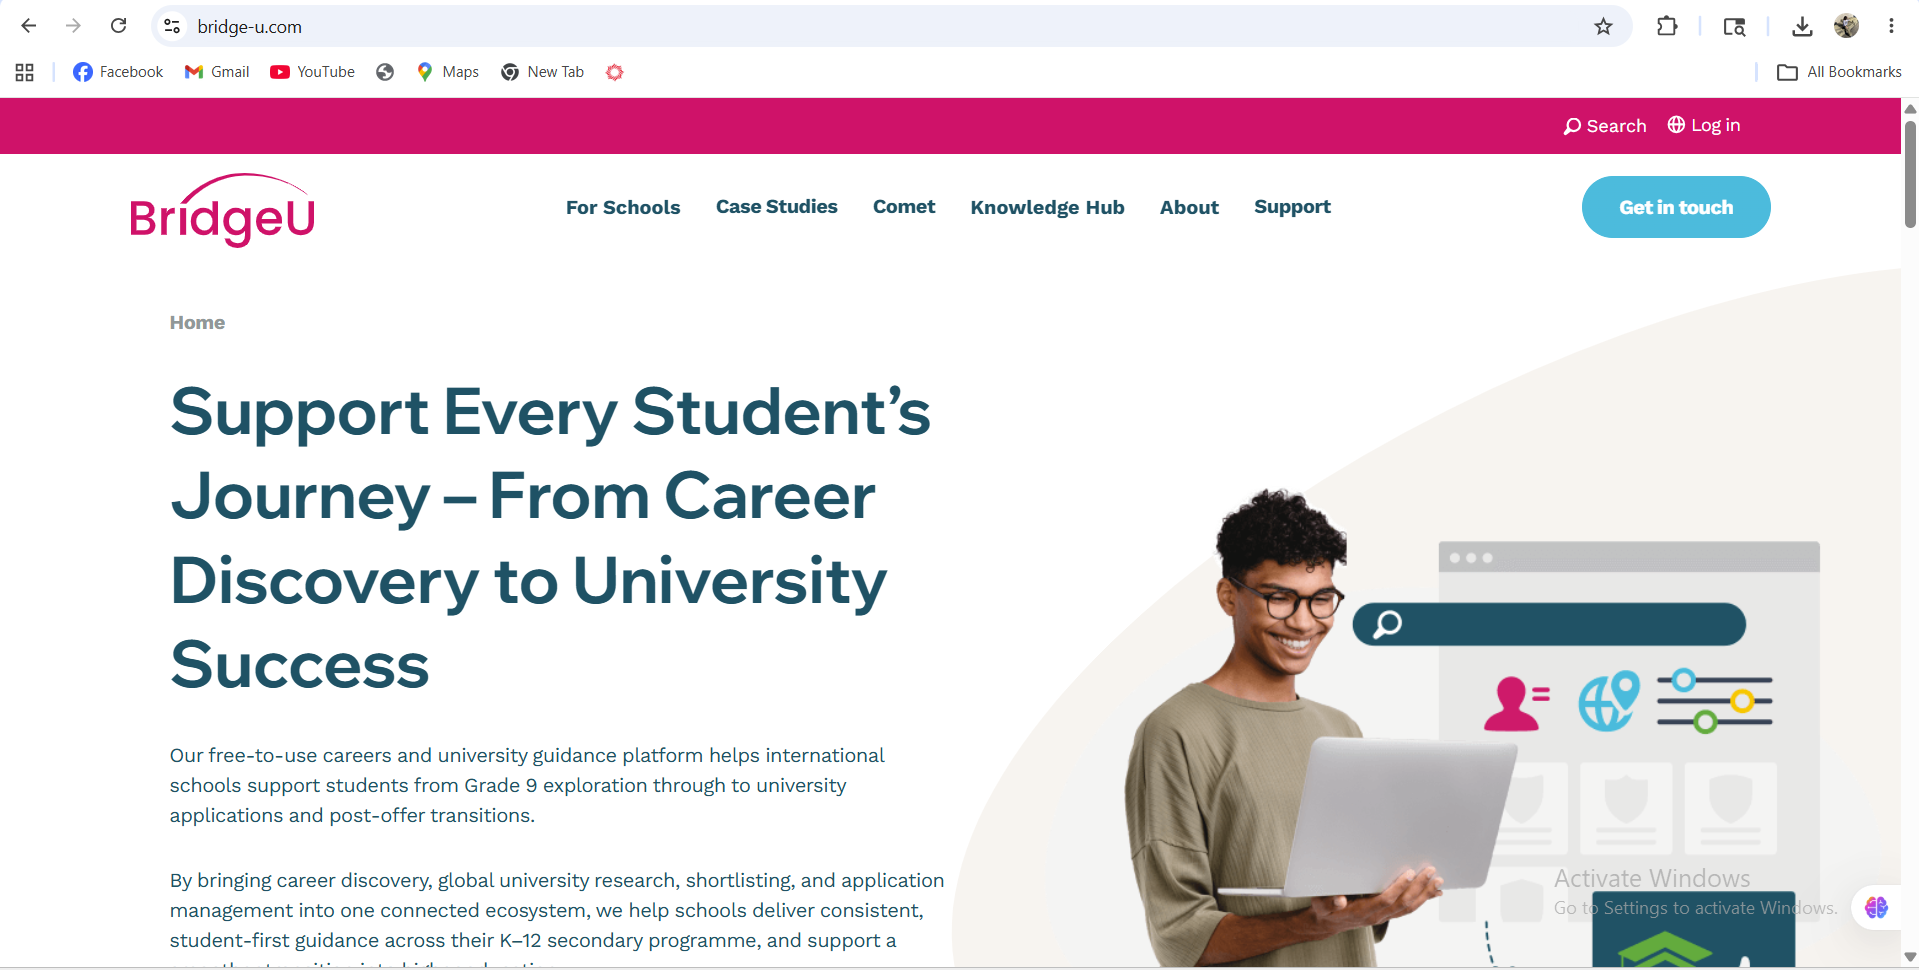
\includegraphics[width=0.9\textwidth]{Figures/chapter1/bridgeu.png}
\caption{BridgeU системийн интерфейс}
\end{figure}

\subsection{Coretech систем}
CoreTech нь Монголд хөгжүүлэгдэж буй college counseling болон application
management чиглэлийн веб платформ бөгөөд дотоодын хэрэглэгчдэд Монгол
хэлээр үйлчилгээ үзүүлэх боломжтойгоороо олон улсын системүүдээс ялгаатай.
Тус систем нь гадаадын их, дээд сургуульд элсэхээр төлөвлөж буй сурагчдад
зөвлөгөө өгөх, элсэлтийн материалын зарим мэдээллийг нэг дор төвлөрүүлэх,
сурагч болон зөвлөхийн хамтын ажиллагааг дэмжих зорилготой платформ гэж
үзэж болно.

CoreTech системийн гол давуу тал нь Монголын боловсролын орчин, хэрэглэгчийн
хэлний хэрэгцээ болон зөвлөх үйлчилгээний практикт илүү ойр байр суурьтай
байгаа явдал юм. Олон улсын Scoir, BridgeU зэрэг системүүдтэй харьцуулахад
Монгол хэрэглэгчдэд ойлгомжтой интерфейс, дотоодын зөвлөх үйлчилгээний
ажлын хэлбэрт нийцэх боломж, хэрэглэгчийн анхан шатны шаардлагыг шууд
тусгах нөхцөл илүү сайн бүрдсэн гэж үзэж болно. Энэ нь Монголын ахлах
сургуулийн сурагчид, зөвлөх багш нарын хувьд системд дасан зохицох хугацааг
бууруулах давуу талтай.

Гэсэн хэдий ч CoreTech системийг судлахад элсэлтийн үйл явцыг бүхэлд нь
системчилсэн байдлаар удирдах боломж хязгаарлагдмал байна. Тухайлбал,
сурагчийн даалгаврын төлөв, материалын хувилбар, дедлайн, тодорхойлох
захидлын хүсэлт, элсэлтийн үр дүн зэрэг мэдээллийг нэг урсгалд холбон
хянах боломж хангалттай хөгжөөгүй. Мөн зөвлөх багш олон сурагчтай зэрэг
ажиллах үед сурагч бүрийн ахиц, хоцрогдол, шаардлагатай дараагийн алхмыг
нэг dashboard-оос харьцуулан харах боломж нь судалж буй системийн
шаардлагатай түвшинд хүрэхгүй байна.

Дээрх ажиглалтыг нэгтгэн үзвэл тус систем нь гадаадын их сургуулийн
элсэлтийн workflow, document tracking, real-time chat болон AI recommendation
зэрэг боломжуудыг бүрэн дэмждэггүй.
Иймээс CoreTech нь Монгол хэл, дотоодын хэрэглэгчийн орчны хувьд давуу талтай
боловч элсэлтийн бэлтгэл ажлыг даалгавар, материал, харилцаа, мэдэгдэл,
хиймэл оюунд суурилсан зөвлөмжтэй уялдуулсан цогц системийн хэрэгцээг
бүрэн хангаж чадахгүй байгаа нь судалгаанаас харагдсан.

\begin{figure}[H]
\centering
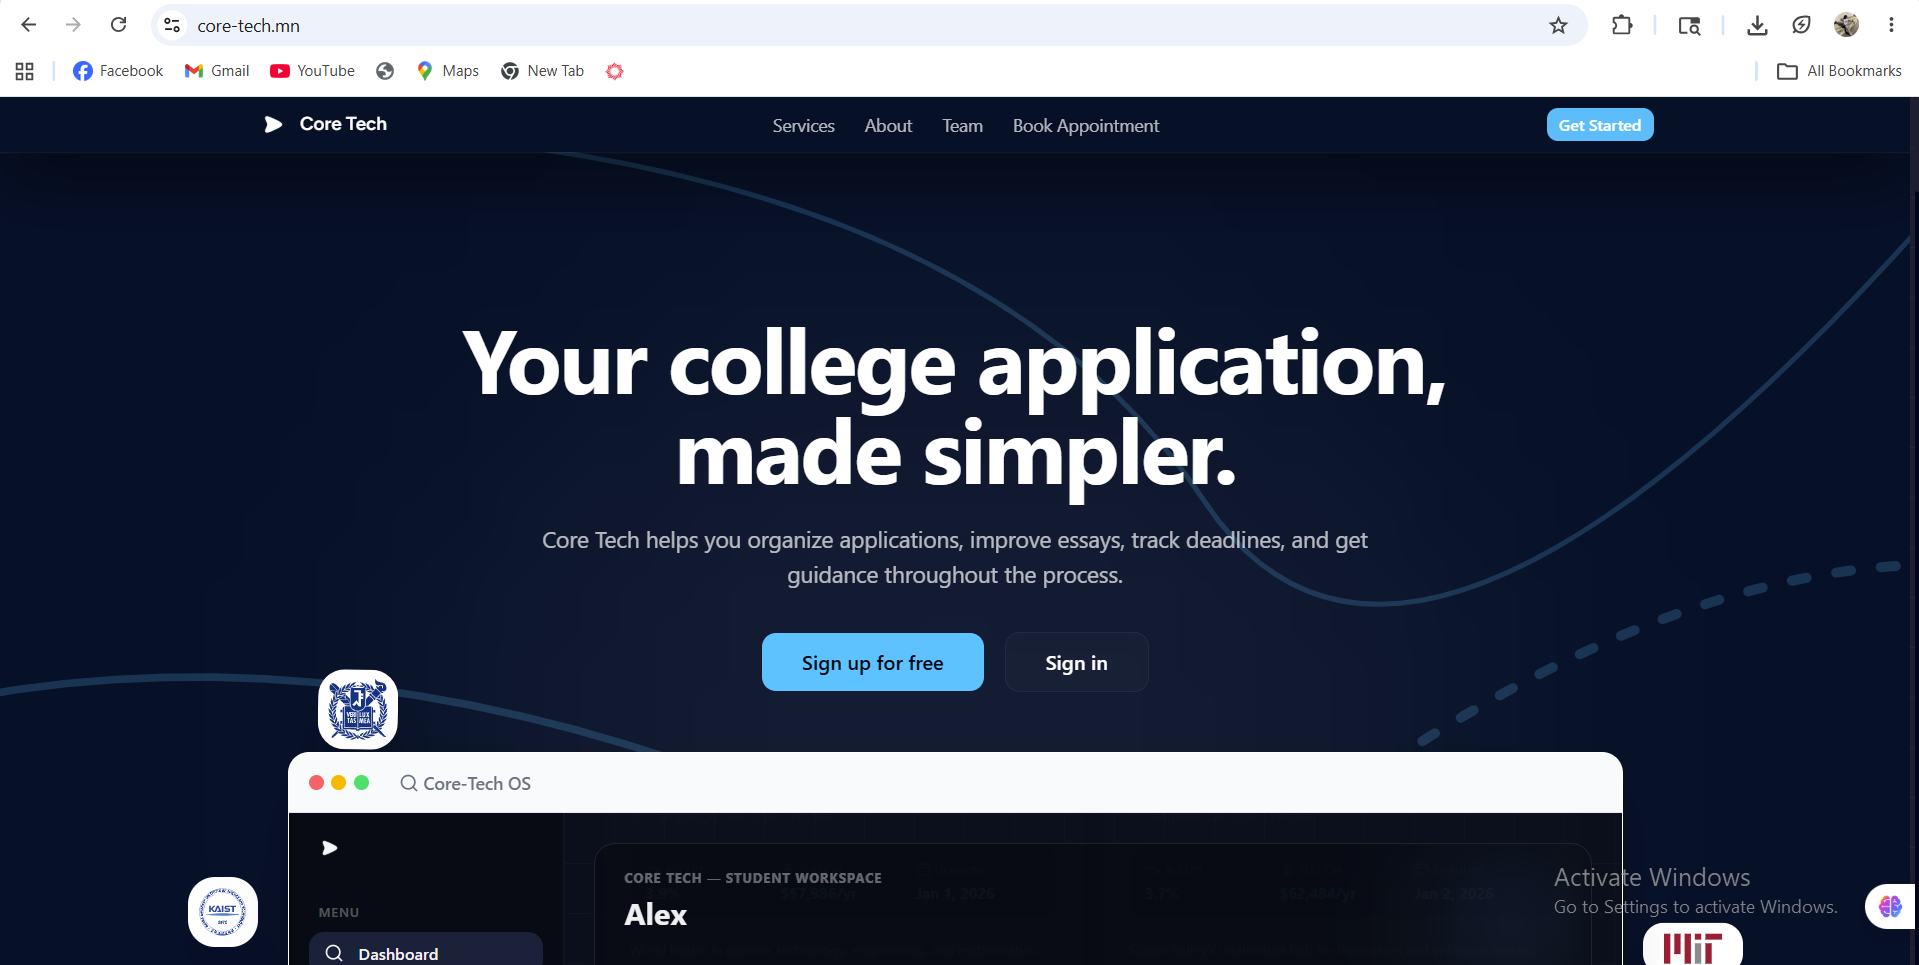
\includegraphics[width=0.9\textwidth]{Figures/chapter1/coretech.png}
\caption{Coretech системийн интерфейс}
\end{figure}

\subsection{Системүүдийн харьцуулалт}

\begin{table}[H]
\centering
\caption{Ижил төстэй системүүдийн харьцуулалт}
{\small
\renewcommand{\arraystretch}{1.25}
\begin{tabular}{|p{4.2cm}|c|c|c|p{4.2cm}|}
\hline
Үзүүлэлт & Scoir & BridgeU & CoreTech & Судалгааны ажиглалт \\
\hline
Даалгаврын удирдлага & Тийм & Тийм & Үгүй & Зөвлөх багш олон сурагчийн явцыг хянахад чухал шаардлагатай. \\
\hline
Бодит цагийн чат & Тийм & Үгүй & Үгүй & Сурагч, зөвлөх багшийн шуурхай харилцааг дэмжих хэрэгцээ байна. \\
\hline
Бичиг баримт байршуулах & Тийм & Тийм & Тийм & Ихэнх системд байгаа боловч материалын хувилбар, төлөвийн хяналт ялгаатай байна. \\
\hline
Хиймэл оюун дэмжих & Тийм & Тийм & Үгүй & Сургуулийн зөвлөмжийг автоматжуулахад ашиглах боломжтой. \\
\hline
Хэрэглэгчийн үүрэгт суурилсан & Тийм & Тийм & Тийм & Сурагч, зөвлөх багш, багш, админы эрхийг ялгах үндсэн шаардлага юм. \\
\hline
Монгол хэлний дэмжлэг & Үгүй & Үгүй & Тийм & Дотоодын хэрэглэгчдэд тохируулахад зайлшгүй шаардлагатай. \\
\hline
И-мэйл сануулга & Тийм & Тийм & Үгүй & Хугацаа хоцрох эрсдэлийг бууруулахад хэрэгтэй. \\
\hline
Элсэлтийн хяналт & Тийм & Тийм & Үгүй & Материал бүрдүүлэлт болон элсэлтийн үр дүнг нэгдсэн байдлаар хянах хэрэгцээ байна. \\
\hline
\end{tabular}
}
\end{table}

Харьцуулалтын үр дүнгээс харахад одоо ашиглагдаж буй системүүд нь зарим
үндсэн боломжуудыг агуулж байгаа боловч Монгол сургуулийн орчинд бүрэн
тохирсон, даалгаврын удирдлага, бодит цагийн чат, хиймэл оюунд суурилсан
зөвлөмж болон элсэлтийн ажлуудыг нэгтгэсэн цогц систем хомс байгаа нь
ажиглагдсан.

\section{Технологийн судалгаа}

Системийг хөгжүүлэхдээ орчин үеийн веб технологи болон үүлэн дэд бүтэцтэй
шийдлүүдийг судалж, системийн шаардлагад нийцсэн технологиудыг сонгон ашигласан.

\subsection{Технологи сонголтын үндэслэл}

Системийн технологийн шийдлийг сонгохдоо хөгжүүлэлтийн хурд, өргөтгөх
боломж, байршуулалтын хялбар байдал, өгөгдлийн бүтэцтэй нийцэх байдал
болон төслийн багийн хэрэгжүүлэх боломжийг харгалзан үзсэн. Доорх
хүснэгтүүдэд frontend framework, өгөгдлийн сан болон байршуулалтын
платформуудыг харьцуулан үзүүлэв.

\begin{table}[H]
\centering
\caption{Frontend технологийн харьцуулалт}
\label{tab:frontend-tech-comparison}
{\small
\setlength{\tabcolsep}{4pt}
\renewcommand{\arraystretch}{1.25}
\begin{tabular}{|p{2.7cm}|p{3.3cm}|p{3.3cm}|p{3.3cm}|}
\hline
\textbf{Үзүүлэлт} & \textbf{Next.js} & \textbf{React SPA} & \textbf{Angular} \\
\hline
Архитектур & Full-stack framework, routing болон API Routes дэмжинэ. & Зөвхөн client-side application хэлбэрээр ажиллах нь түгээмэл. & Бүрэн framework боловч бүтэц, тохиргоо харьцангуй том. \\
\hline
Гүйцэтгэл & Server-side rendering болон static optimization ашиглах боломжтой. & Анхны ачаалалт ихсэх эрсдэлтэй. & Том application-д тохиромжтой боловч эхний тохиргоо их. \\
\hline
Backend уялдаа & Нэг codebase дотор API боловсруулах боломжтой. & Backend-ийг тусад нь зохион байгуулах шаардлагатай. & Backend тусдаа байх шаардлагатай. \\
\hline
Төсөлд нийцэх байдал & Frontend, backend API болон Vercel deployment-тэй сайн нийцнэ. & Энгийн интерфейст тохиромжтой боловч full-stack шаардлагад нэмэлт тохиргоо их. & Том баг, enterprise орчинд илүү тохиромжтой. \\
\hline
\end{tabular}
}
\end{table}

\begin{table}[H]
\centering
\caption{Өгөгдлийн сангийн технологийн харьцуулалт}
\label{tab:database-tech-comparison}
{\small
\setlength{\tabcolsep}{4pt}
\renewcommand{\arraystretch}{1.25}
\begin{tabular}{|p{2.7cm}|p{3.3cm}|p{3.3cm}|p{3.3cm}|}
\hline
\textbf{Үзүүлэлт} & \textbf{MongoDB} & \textbf{PostgreSQL} & \textbf{MySQL} \\
\hline
Өгөгдлийн бүтэц & Уян хатан document бүтэцтэй. & Харилцааны өгөгдөл, complex query-д хүчтэй. & Харилцааны өгөгдөлд тохиромжтой, өргөн хэрэглээтэй. \\
\hline
Схемийн өөрчлөлт & Сурагчийн профайл, файл, чат, AI зөвлөмж зэрэг өөр бүтэцтэй өгөгдөлд уян хатан. & Схемийн өөрчлөлт migration шаарддаг. & Схемийн өөрчлөлт migration шаарддаг. \\
\hline
Node.js уялдаа & Mongoose ODM ашиглан хурдан хөгжүүлэх боломжтой. & ORM ашиглах шаардлагатай. & ORM ашиглах шаардлагатай. \\
\hline
Төсөлд нийцэх байдал & Хэрэглэгч, даалгавар, файл, чат, мэдэгдлийн document өгөгдөлд тохиромжтой. & Нарийн relational transaction давамгай системд илүү тохиромжтой. & Энгийн relational өгөгдөлд тохиромжтой боловч уян хатан document бүтэц сул. \\
\hline
\end{tabular}
}
\end{table}

\begin{table}[H]
\centering
\caption{Байршуулалтын платформын харьцуулалт}
\label{tab:deployment-tech-comparison}
{\small
\setlength{\tabcolsep}{4pt}
\renewcommand{\arraystretch}{1.25}
\begin{tabular}{|p{2.7cm}|p{3.3cm}|p{3.3cm}|p{3.3cm}|}
\hline
\textbf{Үзүүлэлт} & \textbf{Vercel} & \textbf{AWS} & \textbf{Railway} \\
\hline
Next.js дэмжлэг & Next.js-д зориулсан native deployment орчинтой. & Тохируулах боломжтой боловч үйлчилгээ тус бүрийг гараар зохион байгуулах шаардлагатай. & Байршуулахад хялбар боловч Next.js-ийн бүх боломж Vercel шиг нягт уялдаагүй. \\
\hline
CI/CD & GitHub-тэй шууд холбогдож автоматаар байршуулна. & CodePipeline зэрэг нэмэлт тохиргоо шаардана. & GitHub deployment дэмждэг. \\
\hline
Serverless API & API Routes-ийг serverless function хэлбэрээр ажиллуулна. & Lambda, API Gateway зэрэг тусдаа тохиргоо шаарддаг. & Backend service ажиллуулахад тохиромжтой. \\
\hline
Төсөлд нийцэх байдал & Жижиг, дунд хэмжээний Next.js веб системийг хурдан, найдвартай байрлуулахад тохиромжтой. & Том хэмжээний enterprise дэд бүтэц шаардсан үед илүү тохиромжтой. & Туршилт болон хурдан prototype-д тохиромжтой. \\
\hline
\end{tabular}
}
\end{table}

Эдгээр харьцуулалтад үндэслэн Next.js нь frontend болон backend API-г нэг
төслийн хүрээнд зохион байгуулах, Vercel дээр шууд байрлуулах боломжтой
тул энэхүү системд тохиромжтой гэж үзэв. MongoDB нь сурагчийн профайл,
даалгавар, файл, чат, мэдэгдэл болон AI зөвлөмж зэрэг бүтэц нь өөр өөр
өгөгдлийг уян хатан хадгалахад нийцэж байна. Vercel нь Next.js application,
serverless API, Cron Jobs, HTTPS болон CI/CD deployment-ийг нэгтгэн
дэмждэг тул төслийн хэрэгжилт, байршуулалт, засвар үйлчилгээг хялбаршуулна.

\subsection{Frontend технологи}

\subsubsection{Next.js 15}

Next.js нь Vercel компанийн боловсруулсан React framework дээр суурилсан
full-stack веб хөгжүүлэлтийн хэрэгсэл юм. Уг framework нь серверийн талд
хуудас үүсгэх (Server-Side Rendering), статик хуудас үүсгэх (Static Site
Generation), мөн App Router architecture зэрэг орчин үеийн боломжуудыг
дэмждэг.

Энэхүү төсөлд Next.js 15-ийн App Router architecture ашигласан бөгөөд
энэ нь файлын бүтцэд тулгуурлан чиглүүлэлт хийдэг, серверийн болон
клиентийн компонентуудыг тусад нь зохицуулдаг давуу талтай. Мөн нэг
codebase дотор frontend болон backend хоёуланг нь боловсруулах боломж
олгодог тул хөгжүүлэлтийн нарийн төвөгтэй байдлыг эрс бууруулсан.

\subsubsection{Tailwind CSS}

Tailwind CSS нь utility-first буюу нэгж дээр суурилсан CSS framework юм.
Уламжлалт CSS хөгжүүлэлтийн хандлагаас ялгаатай нь HTML дотроо
урьдчилан тодорхойлсон utility class ашиглан загварчлал хийдэг онцлогтой.
Энэ нь дизайны тогтвортой байдлыг хангаж, responsive буюу дэлгэцийн
хэмжээнд дасан зохицдог интерфейс хөгжүүлэх ажлыг хялбаршуулдаг.

Системийн бүх хуудасны загварчлалд Tailwind CSS ашигласан бөгөөд
өнгөний систем, зай, дугуйрсан хүрээ зэргийг нэгдсэн байдлаар
тохируулснаар дизайны нийцтэй байдлыг хангасан.

\subsubsection{Lucide React}

Lucide React нь нээлттэй эхтэй SVG icon санг React компонент хэлбэрээр
ашиглах боломж олгодог хөнгөн жинтэй библиотек юм. Тус библиотекийн
дүрс тэмдгүүд нь цэвэр зураасан дизайнтай, хэмжээ өөрчлөхөд чанараа
хадгалдаг SVG формат дээр суурилсан. Системийн хэрэглэгчийн интерфейсийн
бүх дүрс тэмдгүүдийг Lucide React ашиглан боловсруулсан.

\subsection{Backend технологи}

\subsubsection{Next.js API маршрутууд}

Next.js API Routes нь тус framework-ийн нэг хэсэг бөгөөд
\texttt{app/api} хавтас дотор файл үүсгэснээр REST API цэгүүдийг
тодорхойлох боломж олгодог. Энэ нь тусдаа backend сервер ажиллуулах
шаардлагагүйгээр GET, POST, PATCH, DELETE зэрэг HTTP аргуудыг дэмжсэн
API боловсруулах давуу талтай.

Системд нийт 20 гаруй API цэг боловсруулсан бөгөөд хэрэглэгчийн
нэвтрэлт, даалгавар удирдлага, баримт бичиг байршуулах, зөвлөмж захидал,
чат, мэдэгдэл зэрэг бүх үйлдлийг дэмжиж байна.

\subsubsection{MongoDB ба Mongoose}

MongoDB нь баримт бичигт суурилсан (document-oriented) NoSQL өгөгдлийн
сан бөгөөд өгөгдлийг JSON-тэй төстэй BSON форматаар хадгалдаг.
Уламжлалт харилцааны өгөгдлийн сантай (SQL) харьцуулахад уян хатан
схем дэмжих, хэвтээ өргөтгөл (horizontal scaling) хийх боломж, мөн
объект хэлбэртэй өгөгдөлтэй ажиллахад илүү тохиромжтой зэрэг давуу
талтай.

Mongoose нь MongoDB-тэй Node.js орчинд ажиллах ODM (Object Data Modeling)
библиотек юм. Схем тодорхойлох, өгөгдлийг баталгаажуулах (validation),
дундын үйлдэл (middleware) тохируулах зэрэг боломжуудаар өгөгдөлтэй
ажиллах ажлыг хялбаршуулдаг.

Системд нийт 10 өгөгдлийн загвар боловсруулсан: хэрэглэгч, даалгавар,
баримт бичиг, зөвлөмж захидлын хүсэлт, элсэлтийн үр дүн, карьерын
тест, байгууллага, яриа, мессеж, мэдэгдэл.

\subsubsection{JWT нэвтрэлт}

JWT (JSON Web Token) нь нэвтрэлт болон зөвшөөрлийн мэдээллийг JSON
форматаар кодчилж, дижитал гарын үсгээр баталгаажуулдаг нээлттэй
стандарт (RFC 7519) юм. Сервер хэрэглэгч амжилттай нэвтэрсний дараа
токен үүсгэж, дараагийн хүсэлт бүрт тухайн хэрэглэгчийг таних зориулалтаар
ашигладаг.

Системд httpOnly cookie ашиглан токен хадгалсан нь JavaScript-ээр
токенд хандах боломжгүй болгосноор XSS дайралтаас хамгаалалтыг
нэмэгдүүлсэн. Нэвтрэлтийн токенд хэрэглэгчийн дугаар, үүрэг, нэр,
и-мэйл зэрэг мэдээллийг хадгалдаг бөгөөд 7 хоногийн хүчинтэй хугацааг
тохируулсан.

\subsubsection{bcryptjs}

bcryptjs нь нууц үгийг нэг чиглэлтэй (one-way) hash алгоритмаар
хамгаалах зориулалтын библиотек юм. bcrypt алгоритм нь salt нэмж
боловсруулдаг тул ижил нууц үгийг удаа дараа хашилтад ялгаатай үр дүн
гардаг бөгөөд энэ нь rainbow table дайралтаас хамгаалдаг. Системд
нууц үг хадгалах бүрт 12 давталтын хүч ашигладаг.

\subsection{Үүлэн технологи}

\subsubsection{Vercel}

Vercel нь Next.js-ийг анх боловсруулсан компани бөгөөд тус framework-т
зориулсан хамгийн тохиромжтой байршуулалтын платформ юм. GitHub
репозиторитой шууд холбогдон кодын өөрчлөлт бүрт автоматаар байршуулалт
хийдэг CI/CD боломжтой. Serverless function хэлбэрээр API маршрутуудыг
ажиллуулдаг тул серверийн удирдлага шаардлагагүй бөгөөд ачааллын
дагуу автоматаар өргөтгөгддөг.

\subsubsection{MongoDB Atlas}

MongoDB Atlas нь MongoDB өгөгдлийн санг үүлэн орчинд үйлчилгээ хэлбэрээр
(Database-as-a-Service) санал болгодог платформ юм. Автомат нөөцлөлт
(backup), гэмтэлд тэсвэртэй кластер (replica set), хандалтын хяналт
(IP whitelist, нэвтрэлтийн мэдээлэл), мөн дэлхийн өнцөг булан бүрт байрлах
дата төвүүд зэрэг давуу талтай. Системийн өгөгдлийн санг AWS
Сеул бүсэд байрлуулсан нь Монголоос хандах хоцролтыг бууруулж байна.

\subsubsection{Vercel Blob}

Vercel Blob нь Vercel платформ дээр файл хадгалах үүлэн үйлчилгээ юм.
Сурагчдын байршуулсан CV, эссэ, тодорхойлох бичиг зэрэг баримт бичгүүдийг
энэхүү үйлчилгээнд хадгалдаг. Файлуудыг нийтэд хандах боломжтой URL-аар
хуваалцах, татаж авах боломжтой бөгөөд хэмжээний хязгаарлалтыг API
түвшинд шалгадаг.

\subsubsection{Vercel Cron Jobs}

Vercel Cron Jobs нь тогтмол цагийн хуваарийн дагуу API цэг дуудах
автоматжуулалтын боломж юм. Системд сурагчийн даалгаврын дедлайнаас
тодорхой хоногийн өмнө и-мэйл сануулга илгээх үйлдлийг өдөр бүр өглөөний
08:00 цагт ажиллуулахаар тохируулсан. Cron ажлуудыг зөвшөөрөлгүй дуудахаас
хамгаалах зорилгоор нууц токен баталгаажуулалтыг нэмсэн.

\subsection{Хиймэл оюуны технологи}

\subsubsection{OpenAI GPT-4o-mini}

OpenAI-н GPT-4o-mini нь хурдан хариу өгдөг, зардал хэмнэлттэй томоохон
хэлний загвар юм. Системд сурагчийн сонирхол, академик амжилт, карьерын
тестийн үр дүн зэрэг мэдээлэлд тулгуурлан их сургуулийн зөвлөмж санал
болгоход ашигладаг. API-аар дамжуулан системчилсэн зааварчилгаа болон
сурагчийн мэдээллийг загварт дамжуулж, бүтэцтэй зөвлөмж хүлээн авдаг.

\subsection{Бодит цагийн харилцаа}

Бодит цагийн харилцааны хэрэгцээнд WebSocket технологийн оронд polling
architecture сонгосон. Polling нь серверт тогтмол хугацаанд хүсэлт
илгээн шинэ мэдээлэл байгаа эсэхийг шалгадаг энгийн арга юм.

Чат системд 3 секунд тутамд шинэ мессеж байгаа эсэхийг шалгах хүсэлт
илгээдэг бөгөөд мессежийн цагийн тэмдэглэгээ (timestamp) ашиглан зөвхөн
шинэ мессежийг татаж авдаг тул сүлжээний ачааллыг бууруулсан. Мэдэгдлийн
систем 30 секунд тутам шинэчлэгддэг. WebSocket-тэй харьцуулахад polling нь
хэрэгжүүлэхэд хялбар, serverless орчинд сайн нийцдэг давуу талтай.

% \begin{figure}[H]
% \centering
% \includegraphics[width=0.85\textwidth]{images/system-architecture.png}
% \caption{Системийн архитектур}
% \end{figure}

\section{Бүлгийн дүгнэлт}

Энэхүү бүлэгт гадаадын их, дээд сургуулийн элсэлтийн үйл явцыг удирдах
системийн онолын үндэс, хэрэглэгчийн хэрэгцээ шаардлага, ижил төстэй
системүүд болон хэрэгжүүлэлтэд ашиглах технологийн шийдлүүдийг судаллаа.

Хэрэглэгчийн судалгааны үр дүнгээс харахад элсэлтийн материал бүрдүүлэх
үйл явцад хугацаа удирдах, олон төрлийн материалыг эмх цэгцтэй хадгалах,
даалгаврын биелэлтийг хянах, зөвлөх багштай тогтмол харилцах хэрэгцээ
түгээмэл байна. Одоогийн байдлаар эдгээр ажлыг Excel, Google Sheets, Notion,
чат болон бусад салангид хэрэгслээр гүйцэтгэж байгаа нь мэдээллийн
нэгдмэл байдал алдагдах, материалын хувилбар холилдох, хугацааны сануулга
орхигдох эрсдэлийг нэмэгдүүлж байна. Өөрөөр хэлбэл, одоогийн admission
counseling workflow нь олон хэрэгсэлд хуваагдсан, мэдээллийн урсгал
төвлөрөөгүй, зөвлөх багш болон сурагчийн хамтын ажиллагааг тогтвортой
дэмжихэд хангалтгүй байна.

Ижил төстэй системүүдийн судалгаагаар Scoir болон BridgeU нь олон улсын
түвшинд элсэлтийн зөвлөгөө, сургуулийн санал болголт, материалын хяналтын
боломжуудыг тодорхой хэмжээнд хөгжүүлсэн боловч Монгол хэл, дотоодын
сургуулийн ажлын урсгал, зөвлөх үйлчилгээний онцлогт бүрэн нийцэхгүй
байна. Харин CoreTech нь Монгол хэрэглэгчийн орчинд илүү ойр давуу талтай
боловч даалгаврын удирдлага, real-time chat, document tracking, элсэлтийн
үр дүнгийн хяналт болон AI recommendation зэрэг боломжуудыг нэгтгэсэн
цогц шийдэл болж хараахан бүрдээгүй байна. Иймээс эдгээр системүүдийн
ашигтай функцүүдийг судалгааны эх үүсвэр болгон авч үзэж болох боловч
Монголын ахлах сургуулийн зөвлөх үйлчилгээний ажлын урсгалд шууд бүрэн
нийцнэ гэж үзэх боломжгүй юм.

Иймд судалгааны үндсэн дүгнэлт нь Монголын ахлах сургуулийн сурагч болон
зөвлөх багшид зориулсан, элсэлтийн бэлтгэлийн мэдээллийг төвлөрүүлж,
хэрэглэгчийн үүрэгт суурилсан хандалтын эрхтэй, даалгавар, баримт бичиг,
чат, тодорхойлох захидлын хүсэлт, хиймэл оюунд суурилсан сургуулийн
зөвлөмж болон тайлангийн модулиудыг нэг платформд уялдуулах локалчлагдсан
веб систем шаардлагатай гэсэн дүгнэлт юм. Энэхүү шаардлагыг хангахын тулд
Next.js, MongoDB, JWT, Vercel, Vercel Blob, Vercel Cron Jobs болон хиймэл
оюунд суурилсан зөвлөмжийн технологийг сонгон ашиглах нь системийн ажиллагаа,
өргөтгөх боломж, хэрэглэгчийн аюулгүй байдлын шаардлагад нийцнэ гэж үзэв.
% !TeX root = ../main.tex
